\documentclass{beamer}
\usepackage[utf8]{inputenc}
\usepackage[czech]{babel}
\usepackage[IL2]{fontenc}
\usepackage{amsthm}
\newtheorem{def1}{Definice}

\usetheme{Berkeley}
\usecolortheme{dolphin}


\title{Konečné automaty}


\author{Kamil Vojanec}


\institute[Vysoké učení technické] 
{Fakulta informačních technologií \\ Vysoké učení technické v Brně}

\subject{Finite state machines}

\begin{document}

\begin{frame}
  \titlepage
\end{frame}

\begin{frame}{Obsah prezentace}
  \tableofcontents
\end{frame}


\section{Úvod}


\begin{frame}{Úvod}{Co je to konečný automat?}
  \begin{itemize}
  \item {Výpočetní model}
  \item {HW i SW implementace}
  \item {Simuluje sekvenční logiku}
  \end{itemize}
\end{frame}


\begin{frame}{Úvod}{Formální definice}
    \begin{def1}
        \begin{itemize}
            \item {Konečný stavový automat je pětice $\langle Q, \Sigma, \delta, q_0, F \rangle$, kde:}
            \begin{itemize}
                \item Q \textup{je} konečná množina stavů
                \item $\Sigma$ \textup{je} abeceda
                \item $\delta : Q \times \Sigma \rightarrow Q$ \textup{je} přechodová funkce
                \item $q_0 \in Q$ \textup{je} počáteční stav
                \item $F \subseteq Q$ \textup{je} množina koncových stavů
            \end{itemize}
  
        \end{itemize}
    \end{def1}
\end{frame}



\section{Mealy \& Moore}
\begin{frame}{Mealyho a Mooreův automat}{Rozdíly}
    \begin{block}{Mooreův automat}
        Změna na vstupu se objeví až v následujícím stavu. Závisí pouze na vnitřním stavu
    \end{block}
    \begin{block}{Mealyho automat}
        Na rozdíl od Mooreova automatu závisí kromě vnitřního stavu ještě na příchozím vstupu
    \end{block}

\end{frame}

\section{Příklad -- Moore}
\begin{frame}{Příklad -- Mooreův automat}{Slova končící jedničkou}
  \begin{figure}[h]
      \centering
      \includegraphics[scale=0.25]{citac_moore.png}
      \caption{Automat začíná ve stavu 000 a mění své stavy pouze v závislosti na nich. Na vstupech nezáleží}
      \label{fig:my_label}
  \end{figure}
\end{frame}

\section{Příklad -- Mealy}
\begin{frame}{Příklad -- Mealyho automat}{Slova končící jedničkou}
  \begin{figure}
      \centering
      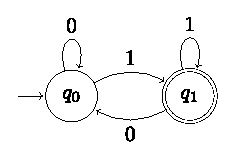
\includegraphics[scale=2]{fsm.eps}
      \caption{Automat se po přijetí znaku 1 přesune z počátečního stavu $q_0$ do stavu $q_1$, a tam setrvá do přijetí znaku 0}
      \label{fig:my_label}
  \end{figure}
\end{frame}


\section{Shrnutí}

\begin{frame}{Shrnutí}
  \begin{itemize}
  \item
    Existují dva typy sutomatů -- Mealyho a Mooreův
  \item
    Reprezentuje všechny stavy systému
  \item
    Implementuje se v SW iHW
  \end{itemize}
  

\end{frame}
\appendix
\section*{\appendixname}
\subsection*{Zdroje}

\begin{frame}{Zdroje}
  \begin{itemize}
      \item \url{https://matematika.cz/konecny-automat}
      \item \url{https://brilliant.org/wiki/finite-state-machines/}
      \item \url{http://www.i-programmer.info/babbages-bag/223-finite-state-machines.html}
      \item Studijní materiály předmětu INC na FIT VUT v Brně
  \end{itemize}
    
\end{frame}

\end{document}


